%%%%%%%%%%%%%%%%%%%%%%%%%%%%%%%%%%%%%%%%%
% Masters/Doctoral Thesis 
% LaTeX Template
% Version 2.5 (27/8/17)
%
% This template was downloaded from:
% http://www.LaTeXTemplates.com
%
% Version 2.x major modifications by:
% Vel (vel@latextemplates.com)
%
% This template is based on a template by:
% Steve Gunn (http://users.ecs.soton.ac.uk/srg/softwaretools/document/templates/)
% Sunil Patel (http://www.sunilpatel.co.uk/thesis-template/)
%
% Template license:
% CC BY-NC-SA 3.0 (http://creativecommons.org/licenses/by-nc-sa/3.0/)
%
%%%%%%%%%%%%%%%%%%%%%%%%%%%%%%%%%%%%%%%%%

%----------------------------------------------------------------------------------------
%	PACKAGES AND OTHER DOCUMENT CONFIGURATIONS
%----------------------------------------------------------------------------------------

\documentclass[
12pt, % The default document font size, options: 10pt, 11pt, 12pt
%oneside, % Two side (alternating margins) for binding by default, uncomment to switch to one side
oneside,
english, % ngerman for German
singlespacing, % Single line spacing, alternatives: onehalfspacing or doublespacing
%draft, % Uncomment to enable draft mode (no pictures, no links, overfull hboxes indicated)
%nolistspacing, % If the document is onehalfspacing or doublespacing, uncomment this to set spacing in lists to single
%liststotoc, % Uncomment to add the list of figures/tables/etc to the table of contents
%toctotoc, % Uncomment to add the main table of contents to the table of contents
%parskip, % Uncomment to add space between paragraphs
%nohyperref, % Uncomment to not load the hyperref package
headsepline, % Uncomment to get a line under the header
%chapterinoneline, % Uncomment to place the chapter title next to the number on one line
%consistentlayout, % Uncomment to change the layout of the declaration, abstract and acknowledgements pages to match the default layout
]{MastersDoctoralThesis}% The class file specifying the document structure%

\usepackage{polyglossia}
\usepackage{amsmath,amssymb,amsfonts}
\newcommand{\familytype}{} %new commit
\setmainlanguage{english}
\setotherlanguage{hindi}

\newfontfamily\devanagarifont[Script=Devanagari]{Noto Serif Devanagari}
\linespread{1.25}

\usepackage[utf8]{inputenc} % Required for inputting international characters
\usepackage[T1]{fontenc} % Output font encoding for international characters

\usepackage{mathpazo} % Use the Palatino font by default

\usepackage[backend=bibtex,style=ieee,natbib=true]{biblatex} % Use the bibtex backend with the authoryear citation style (which resembles APA)

\addbibresource{References.bib} % The filename of the bibliography

\usepackage[autostyle=true]{csquotes} % Required to generate language-dependent quotes in the bibliography

%----------------------------------------------------------------------------------------
%	MARGIN SETTINGS
%----------------------------------------------------------------------------------------
\geometry{
	paper=a4paper, % Change to letterpaper for US letter
	inner=2.5cm, % Inner margin
	outer=2.5cm, % Outer margin
	bindingoffset=.5cm, % Binding offset
	top=1.5cm, % Top margin
	bottom=2.2cm, % Bottom margin
	%showframe, % Uncomment to show how the type block is set on the page
}

%----------------------------------------------------------------------------------------
%	THESIS INFORMATION
%----------------------------------------------------------------------------------------

\thesistitle{report title} % Your thesis title, this is used in the title and abstract, print it elsewhere with \ttitle
\supervisor{Dr. Vipin Kumar} % Your supervisor's name, this is used in the title page, print it elsewhere with \supname
\examiner{} % Your examiner's name, this is not currently used anywhere in the template, print it elsewhere with \examname
\degree{\uppercase{\textbf{Master of Techonolgy}}} % Your degree name, this is used in the title page and abstract, print it elsewhere with \degreename
\author{Subham Kumar\\ (MGCU2021CSIT4029)} % Your name, this is used in the title page and abstract, print it elsewhere with \authorname
\addresses{} % Your address, this is not currently used anywhere in the template, print it elsewhere with \addressname

\subject{Computer Science \& Engineering} % Your subject area, this is not currently used anywhere in the template, print it elsewhere with \subjectname
\keywords{} % Keywords for your thesis, this is not currently used anywhere in the template, print it elsewhere with \keywordnames
\university{\href{https://mgcub.ac.in}{Mahatma Gandhi Central University, Motihari, Bihar-845401, India}} % Your university's name and URL, this is used in the title page and abstract, print it elsewhere with \univname
\department{\href{https://mgcub.ac.in/department_of_computer_science.php}{DEPARTMENT OF COMPUTER SCIENCE AND INFORMATION TECHNOLOGY}} % Your department's name and URL, this is used in the title page and abstract, print it elsewhere with \deptname
\group{\href{http://researchgroup.university.com}{Research Group Name}} % Your research group's name and URL, this is used in the title page, print it elsewhere with \groupname
\faculty{\href{https://mgcub.ac.in/department_of_computer_science_faculty.php}{Dr. Vipin Kumar}} % Your faculty's name and URL, this is used in the title page and abstract, print it elsewhere with \facname

\AtBeginDocument{
\hypersetup{pdftitle=\ttitle} % Set the PDF's title to your title
\hypersetup{pdfauthor=\authorname} % Set the PDF's author to your name
\hypersetup{pdfkeywords=\keywordnames} % Set the PDF's keywords to your keywords
}
\usepackage{Edit}
\usepackage{ragged2e}
\usepackage{lscape}
 \usepackage{booktabs}
 \usepackage{graphicx}
 \usepackage{float}




\justifying
\begin{document}

\frontmatter % Use roman page numbering style (i, ii, iii, iv...) for the pre-content pages

\pagestyle{plain} % Default to the plain heading style until the thesis style is called for the body content


%--------------------cover----------------------
%----------------------------------------------------------------------------------------
%	COVER PAGE
%----------------------------------------------------------------------------------------

\begin{titlepage}
\begin{center}

%\vspace*{.06\textheight}

%\textsc{\Large Masters Thesis}\\[0.5cm] % Thesis type

%\HRule \\[0.4cm] % Horizontal line
{\LARGE \bfseries \ReportTitel \par}\vspace{0.3cm} % Thesis title
%\HRule \\[1.5cm] % Horizontal line

%\begin{minipage}[t]{0.4\textwidth}
%\begin{flushleft} \large
%%\emph{Author:}\\
%%\href{http://www.johnsmith.com}{\authorname} % Author name - remove the \href bracket to remove the link
%\end{flushleft}
%\end{minipage}
%\begin{minipage}[t]{0.4\textwidth}
%\begin{flushright} \large
%%\emph{Supervisor:} \\
%%\href{http://www.jamessmith.com}{\supname} % Supervisor name - remove the \href bracket to remove the link
%\end{flushright}
%\end{minipage}\\[1cm]
%
\vfill

\large \textit{A \rType  submitted to the \Uni}\\[0cm] % University requirement text
\large \textit{in partially fulfillment of the requirements}\\[0cm]
\large \textit{for the award of the degree of}\\[0cm]

\textbf{\Degree}\\[0cm]

\uppercase{In}\\[0cm]

\uppercase{\textbf{\Cour}}\\[0cm]

\uppercase{By}\\[0cm]

\uppercase{\textbf{\fAuthorC}}\\[1cm]




%   \begin{figure}[H]
        %   \centering
\centerline{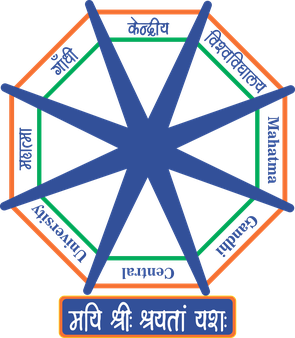
\includegraphics[height=1.5in,width=1.5in, keepaspectratio]{mgcu.png}}
        %   \includegraphics{logo}% logo
    %   \end{figure}
\vfill
\vspace{1cm}
\normalsize{\departmentC}\\[-0.1cm] %search group name and department name
%\school\\[0.1cm]
%\large{\groupname}\\[-0.2cm]

{\scshape\Large \UniversityC \par}\vspace{1cm} % University name%\university\\[2cm]
\vfill

{\large \today}\\[1cm] % Date
%\includegraphics{Logo} % University/department logo - uncomment to place it

\vfill

\end{center}
\end{titlepage}
%--------------------cover----------------------

%--------------------Title----------------------
\begin{titlepage}
\begin{center}

%\vspace*{.06\textheight}

%\textsc{\Large Masters Thesis}\\[0.5cm] % Thesis type

%\HRule \\[0.4cm] % Horizontal line
{\LARGE \bfseries \ReportTitel \par}\vspace{0.1cm} % Thesis title
%\HRule \\[1.5cm] % Horizontal line

%\begin{minipage}[t]{0.4\textwidth}
%\begin{flushleft} \large
%%\emph{Author:}\\
%%\href{http://www.johnsmith.com}{\authorname} % Author name - remove the \href bracket to remove the link
%\end{flushleft}
%\end{minipage}
%\begin{minipage}[t]{0.4\textwidth}
%\begin{flushright} \large
%%\emph{Supervisor:} \\
%%\href{http://www.jamessmith.com}{\supname} % Supervisor name - remove the \href bracket to remove the link
%\end{flushright}
%\end{minipage}\\[1cm]
%
\vfill

\large \textit{A \rType submitted to the \Uni}\\[0cm] % University requirement text
\large \textit{in partially fulfillment of the requirements}\\[0cm]
\large \textit{for the award of the degree of}\\[0cm]

\textbf{\Degree}\\[0cm]

\uppercase{In}\\[0cm]

\uppercase{\textbf{\Cour}}\\[0cm]

\uppercase{By}\\[0cm]

\uppercase{\textbf{\fAuthorC \\[0cm] (\fAID)}}\\[0cm]

\large \textit{Under the Supervision of}\\[0cm]
\uppercase{\textbf{\SupervisorC}}\\[0.3cm]




%   \begin{figure}[H]
        %   \centering
        \centerline{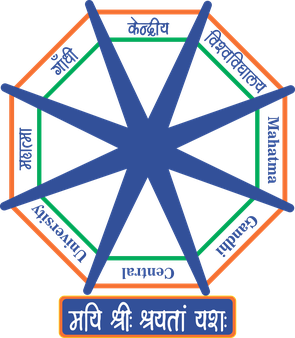
\includegraphics[height=1.5in,width=1.5in, keepaspectratio]{mgcu.png}}
        %   \includegraphics{logo}% logo
    %   \end{figure}
\vfill
\vspace{0.3cm}
\normalsize{\departmentC}\\[-0.1cm] % Research group name and department name
%\school\\[0.01cm]
%\large{\groupname}\\[-0.2cm]

{\scshape\Large \UniversityC \par}\vspace{1cm} % University name%\university\\[2cm]
\vfill

{\large \today}\\[0.1cm] % Date
%\includegraphics{Logo} % University/department logo - uncomment to place it

\vfill
\end{center}
\end{titlepage}

%--------------------Title----------------------
%------------------------declaration------------
%----------------------------------------------------------------------------------------
%	DECLARATION PAGE
%----------------------------------------------------------------------------------------

\chapter*{}
\vspace*{-3.5cm}
% \thispagestyle{empty}

\setlength\tabcolsep{0pt}
\def\arraystretch{0}
\begin{table}[h]
\begin{center}
\begin{tabular}{r  l}
   \begin{minipage}{0.18\textwidth}
\begin{flushleft}
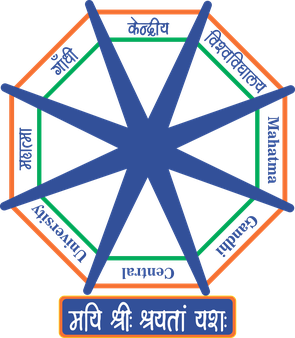
\includegraphics[height=1.25in,width=1.25in, keepaspectratio]{mgcu.png}
\end{flushleft}
\end{minipage}
&
\begin{minipage}{0.83\textwidth}
\begin{flushleft}

\begin{hindi}\Large \centering \departmentH\\
\end{hindi}
\centering\textbf{\department}\\
%\deptname\\[0.01cm] % Research group name and department name
\begin{hindi}\LARGE\centering\textbf{\UniversityH}\\
\end{hindi}
\vspace*{-0.1cm}
{\scshape\large\textbf\centering\UniversityC\par} % University name%\university\\[2cm]
\end{flushleft}
\end{minipage}
\noindent
\\
\end{tabular}
%\label{tab1}
\end{center}
\end{table}


\vspace{2ex}
\addchaptertocentry{\authorshipname} % Add the certificatename to the table of contents
\begin{center}
    \textbf{\LARGE\underline {DECLARATION}}
\end{center}

\vspace{3ex}
This is to certify that the \rType entitled {\bfseries " \ReportTitel "} is being submitted to the
\textbf{\department, \University } in partial fulfillment of
the requirements for the award of the degree of \textbf{\fACourse} in \textbf {Computer Science \& Engineering}, is a record of bonafide work carried out by me under the
supervision of  \textbf{"\Supervisor, \department, \University ."}\\[0.1cm]
\indent The matter embodied in the dissertation has not been submitted in part or full to any
University or Institution for the award of any other degree or diploma.
\par During the preparation of this work, I have not used any AI-based tool to write any part of this dissertation report. I take full responsibility for the submitted content including similarity.
\vspace*{0.55cm}

\setlength\tabcolsep{0pt}
\def\arraystretch{0}
\begin{table}[h]
\begin{center}
\begin{tabular}{r  r}
   \begin{minipage}{0.5\textwidth}
\begin{flushleft}

\end{flushleft}
\end{minipage}
&
\begin{minipage}{0.5\textwidth}
\begin{flushleft}

\vspace*{0.6cm}

\textbf \Author

\department\\[.1cm]
\University\\[.1cm]
Email id: - \fAemail
\end{flushleft}
\end{minipage}
\noindent
\\
\end{tabular}
%\label{tab1}
\end{center}
\end{table}

%\end{declaration}
\cleardoublepage

%------------------------declaration------------
%----------------------------------------------------------------------------------------
%	QUOTATION PAGE
%----------------------------------------------------------------------------------------

\vspace*{0.2\textheight}

\noindent\enquote{\itshape I am enough of an artist to draw freely upon my imagination. Imagination is more important than knowledge. For knowledge is limited, whereas imagination encircles the world.}\bigbreak

\hfill Albert Einstein

%----------------------------------------------------------------------------------------
%	CERTIFICATE
%----------------------------------------------------------------------------------------
\hyphenpenalty 200  %for justifi content
\tolerance 2000
\chapter*{}
\vspace*{-3.5cm}
% \thispagestyle{empty}

\setlength\tabcolsep{0pt}
\def\arraystretch{0}
\begin{table}[h]
\begin{center}
\begin{tabular}{r  l}
   \begin{minipage}{0.18\textwidth}
\begin{flushleft}
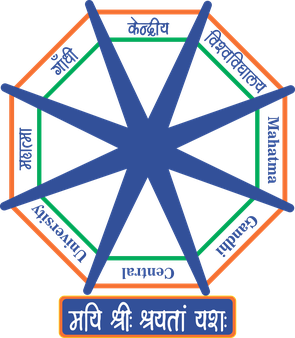
\includegraphics[height=1.25in,width=1.25in, keepaspectratio]{mgcu.png}
\end{flushleft}
\end{minipage}
&
\begin{minipage}{0.83\textwidth}
\begin{flushleft}

\begin{hindi}\Large \centering \departmentH\\
\end{hindi}
\centering\textbf{\department}\\
%\deptname\\[0.01cm] % Research group name and department name
\begin{hindi}\LARGE\centering\textbf{\UniversityH}\\
\end{hindi}
\vspace*{-0.1cm}
{\scshape\large\textbf\centering\UniversityC \par} % University name%\university\\[2cm]
\end{flushleft}
\end{minipage}
\noindent
\\
\end{tabular}
%\label{tab1}
\end{center}
\end{table}



\vspace{4ex}
\addchaptertocentry{\certificatename} % Add the certificatename to the table of contents
\begin{center}
    \textbf{\LARGE\underline {CERTIFICATE}}
\end{center}

\vspace{4ex}

This is to certify that the \rType entitled {\bfseries  "\ReportTitel"} submitted by \textbf {\fAuthor} to the
\textbf{\department, \University} for the award of the degree of \textbf{\fACourse} in \textbf{\fATrade}, is a research work carried out by him under the
supervision of  \textbf{"\Supervisor, \department, \University ."}\\[0.1cm]

\vspace*{1cm}

\setlength\tabcolsep{0pt}
\def\arraystretch{0}
\begin{table}[h]
\begin{center}
\begin{tabular}{l  r}
   \begin{minipage}{0.55\textwidth}
\begin{flushleft}
\textbf{Head of Department}\\[.3cm]
\textbf{\HodName}\\[.1cm]

\department\\[.1cm]
\University\\[.1cm]

\end{flushleft}
\end{minipage}
&
\begin{minipage}{0.5\textwidth}
\begin{flushleft}

\textbf{Supervisor}\\[.3cm]
\textbf{\Supervisor}\\[.1cm]

\department\\[.1cm]
\University\\[.1cm]

\end{flushleft}
\end{minipage}
\noindent
\\
\end{tabular}
%\label{tab1}
\end{center}
\end{table}

%----------------------------------------------------------------------------------------
%	ABSTRACT PAGE
%----------------------------------------------------------------------------------------

\begin{abstract}
\addchaptertocentry{\abstractname} % Add the abstract to the table of contents
Paragraph
\end{abstract}

%----------------------------------------------------------------------------------------
%	ACKNOWLEDGEMENTS
%----------------------------------------------------------------------------------------

\begin{acknowledgements}
\addchaptertocentry{\acknowledgementname} % Add the acknowledgements to the table of contents
\vspace*{2cm}
This M.Tech \rType is the result of hard work, upon which many people have contributed and given their support. I
have made this dissertation on the topic \textbf{"\ReportTitel ."} I have also tried my best in this dissertation to
explain all the related detail. I would like to express my sincere gratitude towards my Superviser \textbf{
	\Supervisor}, Department of \depS, for providing excellent guidance, encouragement, inspiration, and constant and
timely support throughout this \DegreeS \  dissertation work. He taught me how to pursue the right aim towards the work
, and showed me differnt ways to approach the research problem. His wide knowledge and logical ways of thinking have
been great value for me, and his understanding and guidance have provided the successful completion of the
Dissertation work.

First and foremost, I would like to express my gratitude to our beloved Dean of the Computational Sciences,
Information and Communication Technology and Head of Department of Computer Science and Information Technology \textbf{\HodName},
for providing his kind support in various aspects. A special thanks to all the Respected Teachers
\textbf{\Facone}, \textbf{\Factwo}, and \textbf{\Facthree}, of the Department of Computer Science and Information
Technology.

I am always grateful to the university, our Hon’ble Vice chancellor \textbf{\Vc} for providing
such a good research environment.

	Special thanks to Ph.D scholar, especially \textbf{Ritika Singh}, \textbf{Surbhi Kumari}, \textbf{Ibrahim Momin},
\textbf{Naushad Ahmad} and  my friends \textbf{Tej Prakash}, \textbf{Gajendra Patel}, \textbf{Abhijeet Kumar},
\textbf{Amod Kumar}, \textbf{Rana Kumar}, \textbf{Krishna Murari}, \textbf{Rajan Kumar}, \textbf{Suraj}, \textbf{Md.
Aamir Sohail}, \textbf{
	Shahzeb Khan},
and all my lovely juniors  for their invaluable feedbacks, care, and moral support during this endeavor.

	\textbf{Mother} and \textbf{Father}, it is impossible to thanks adequately for everything you have done, from
loving me unconditionally to rising me in a stable household, where your persistent efforts and traditional values
taught your children to celebrate and embrace life. I could not have asked for better parents or role-models. You
showed me that anything is possible with faith, hard work and determination. 


\vspace*{0.7cm}

\setlength\tabcolsep{0pt}
\def\arraystretch{0}
\begin{table}[h]
\begin{center}
\begin{tabular}{r  r}
   \begin{minipage}{0.5\textwidth}
\begin{flushleft}
\vspace*{1cm}

\textbf{\fAuthor}\\
\textbf{(\fAID)}\\
\textbf{\DegreeS(CSE)}\\[.1cm]
\end{flushleft}
\end{minipage}
&
\begin{minipage}{0.5\textwidth}
\begin{flushleft}



\end{flushleft}
\end{minipage}
\noindent
\\
\end{tabular}
%\label{tab1}
\end{center}
\end{table}

\end{acknowledgements}

%----------------------------------------------------------------------------------------
%	PUBLICATION PAGE
%----------------------------------------------------------------------------------------

\chapter*{}
\vspace*{-3.5cm}
% \thispagestyle{empty}

\vspace{11ex}
\addchaptertocentry{\listofpublication} % Add the certificatename to the table of contents
%\begin{center}
    \textbf{\huge {List of Publications}}
%\end{center}

\vspace{7ex}



\noindent\textbf{1.titel of publication }\\
publishar \\
Authors - \textbf{\fAuthor} and  Vipin Kumar\\




\vspace*{0.7cm}

%----------------------------------------------------------------------------------------
%	LIST OF CONTENTS/FIGURES/TABLES PAGES


\tableofcontents % Prints the main table of contents


\listoffigures % Prints the list of figures
\addchaptertocentry{\listfigurename} % Add the figurename to the table of contents


\listoftables % Prints the list of tables
\addchaptertocentry{\listtablename} % Add the tablename to the table of contents
%----------------------------------------------------------------------------------------
%----------------------------------------------------------------------------------------
%	ABBREVIATIONS
%----------------------------------------------------------------------------------------
\begin{abbreviations}{ll} % Include a list of abbreviations (a table of two columns)
\addchaptertocentry{\abbrevname} % Add the List of Abbreviations to the table of contents
\vspace*{0.3cm}
%\textbf{LR} & \textbf{L}ist \textbf{A}bbreviations \textbf{H}ere\\
%\vspace*{0.1cm}
\noindent\textbf{ML} & { }{ }{ }{ }{ }{ }{ }{ }{ } \textbf{Machine Learning} \\
\vspace*{0.3cm}
\textbf{DL} & { }{ }{ }{ }{ }{ }{ }{ }{ } \textbf{Deep Learning} \\
\vspace*{0.3cm}
\textbf{CNN} & { }{ }{ }{ }{ }{ }{ }{ }{ } \textbf{Convolutional Neural Network} \\

\vspace*{0.3cm}





\end{abbreviations}


%----------------------------------------------------------------------------------------
%	SYMBOLS
%----------------------------------------------------------------------------------------

\begin{symbols}{lll} % Include a list of Symbols (a three column table)
\addchaptertocentry{\symbolsname} % Add the List of Abbreviations to the table of contents


\vspace*{0.3cm}
$D$ & { }{ }{ }{ }{ }{ }{ }{ }{ } \textbf{Dataset} \\
\vspace*{0.3cm}
$N$ & { }{ }{ }{ }{ }{ }{ }{ }{ } \textbf{Number of data points} \\
\vspace*{0.3cm}
$y(i)$ & { }{ }{ }{ }{ }{ }{ }{ }{ } \textbf{$i^{th}$ measurement} \\


%$P$ & power & \si{\watt} (\si{\joule\per\second}) \\
%Symbol & Name & Unit \\

\addlinespace % Gap to separate the Roman symbols from the Greek

%$\omega$ & angular frequency & \si{\radian} \\

\end{symbols}

%----------------------------------------------------------------------------------------
%	DEDICATION
%----------------------------------------------------------------------------------------

\dedicatory{Dedicated\\ to  \vspace*{0.3cm}          \\ Maa, and Papajee}
%----------------------------------------------------------------------------------------
%	STATEMENT OF THESIS PREPARATION
%----------------------------------------------------------------------------------------
\vspace{4ex}
\addchaptertocentry{\certificatename}

\begin{center}
    \textbf {\Large{STATEMENT OF THESIS PREPARATION}}
\end{center}



\begin{enumerate}
\item Thesis Title:\\
\textbf{"\ReportTitel"}
\item Degree for which the thesis is submitted: \textbf{ \fACourse .}
\item The thesis Guide was referred for preparing the thesis. 
\item Specifications regarding the thesis format have been closely followed. 
\item The contents of the thesis have been organized based on the guidelines. 
\item The thesis has been prepared without resorting to plagiarism. 
\item All sources used have been cited appropriately. 
\item The thesis has not been submitted elsewhere for a degree. 
\item A copy of Research Article submission/Publication Certificate(s)/Proof of Journal/Conference (National/International) based on dissertation work done during the session is mandatory to submit i.e. forwarded by supervisor(s). 


\end{enumerate}






\vspace*{2cm}

\setlength\tabcolsep{0pt}
\def\arraystretch{0}
\begin{table}[h]
\begin{center}
\begin{tabular}{l  r}
\begin{minipage}{0.55\textwidth}
\begin{flushleft}
\end{flushleft}
\end{minipage}
&
\begin{minipage}{0.5\textwidth}
\begin{flushleft}


\textbf{\fAuthorC}\\[.1cm]
Enrolment No.: \fAID \\[.1cm]
\department\\[.1cm]
\University\\[.1cm]
Email id - \fAemail\\[.1cm]

\end{flushleft}
\end{minipage}
\noindent
\\
\end{tabular}
%\label{tab1}
\end{center}
\end{table}

%----------------------------------------------------------------------------------------
%	THESIS CONTENT - CHAPTERS
%----------------------------------------------------------------------------------------

\mainmatter % Begin numeric (1,2,3...) page numbering

\pagestyle{thesis} % Return the page headers back to the "thesis" style

% Include the chapters of the thesis as separate files from the Chapters folder
% Uncomment the lines as you write the chapters

% Chapter Template

\chapter{Introduction} % Main chapter title

\label{c1} % Change X to a consecutive number; for referencing this chapter elsewhere, use \ref{ChapterX}

%----------------------------------------------------------------------------------------
%	SECTION 1
%----------------------------------------------------------------------------------------

\section{Introduction}
\par Paragraph1
\par Paragraph2
\par Paragraph3

% Chapter Template

\chapter{Literature Review} % Main chapter title

\label{c2} % Change X to a consecutive number; for referencing this chapter elsewhere, use \ref{ChapterX}

%----------------------------------------------------------------------------------------
%	SECTION 1
%----------------------------------------------------------------------------------------

\section{Literature Review}

% Please add the following required packages to your document preamble:
% \usepackage{lscape}
% \usepackage{longtable}
% Note: It may be necessary to compile the document several times to get a multi-page table to line up properly

\par Paragraph
\par Paragraph

Table \ref{table:Lr} REFRENCE OF TABLE

\begin{landscape}

\setlength{\tabcolsep}{3pt}

{\renewcommand{\arraystretch}{1}%
\begin{longtable}[c]{|p{0.12\linewidth}|p{0.13\linewidth}|p{0.26\linewidth}|p{0.13\linewidth}|p{0.15\linewidth}|p{0.16\linewidth}|}%{|l|l|l|l|l|l|}
\caption{Summarizing of Related work to pridict $PM_{2.5}$}
\label{table:Lr}
\\ \hline
\textbf{Paper }                      & \textbf{Proposed Model}           & \textbf{Data Source} & \textbf{Forecasting Object}              & \textbf{Benchmark Models }                         & \textbf{Results}
\\ \hline
\endhead
%
&&&&&\\ \hline
...&...&...&...&...&...\\ \hline
\end{longtable}}
\end{landscape}

% Chapter Template

\chapter{Basics Related Roncepts} % Main chapter title

\label{c3} % Change X to a consecutive number; for referencing this chapter elsewhere, use \ref{ChapterX}

%----------------------------------------------------------------------------------------
%	SECTION 1
%----------------------------------------------------------------------------------------
\section{Basics Related Roncepts}
\subsection{Machine Learning}

\par Paragraph




% Chapter Template

\chapter{Methodology} % Main chapter title

\label{c4} % Change X to a consecutive number; for referencing this chapter elsewhere, use \ref{ChapterX}

\section{Methodology}
\pagebreak

\begin{table}[H]
\setlength{\tabcolsep}{3pt}
{\renewcommand{\arraystretch}{1}%
\begin{longtable}[c]{|p{0.28\linewidth}|p{0.20\linewidth}|p{0.20\linewidth}|p{0.22\linewidth}|}%{|l|l|l|l|}
    \caption{17 Indian cities dataset, with start and end dates and sample counts.}
\label{table:Data}
\\ \hline
\textbf{DataSets }  & \textbf{Fast\_Day} & \textbf{Last\_Day} & \textbf{No of Samples}
\\ \hline
\endhead
%
BHIWADI        & 20-12-2017 15:00 & 02-12-2022 16:00 & 43394 \\ \hline
JODHPUR        & 01-12-2015 00:00 & 02-12-2022 16:00 & 61409 \\ \hline
SINGRAULI      & 08-12-2017 11:00 & 03-12-2022 01:00 & 43695 \\ \hline
ANKLESHWAR     & 04-02-2019 18:00 & 03-12-2022 00:00 & 33535 \\ \hline
LUDHIANA       & 01-05-2017 00:00 & 03-12-2022 01:00 & 49010 \\ \hline
DURGAPUR       & 06-12-2020 15:00 & 03-12-2022 00:00 & 17434 \\ \hline
YAMUNA\_NAGAR  & 03-01-2019 14:00 & 02-12-2022 16:00 & 34299 \\ \hline
CHARKHI\_DADRI & 03-03-2020 15:00 & 02-12-2022 17:00 & 24099 \\ \hline
JIND           & 10-01-2019 09:00 & 03-12-2022 01:00 & 34145 \\ \hline
KURUKSHETRA    & 07-01-2019 18:00 & 03-12-2022 01:00 & 34208 \\ \hline
SONIPAT        & 01-01-2019 00:00 & 02-12-2022 17:00 & 34362 \\ \hline
DHARUHERA      & 04-01-2019 12:00 & 02-12-2022 04:00 & 34265 \\ \hline
AMBALA         & 08-01-2019 12:00 & 02-12-2022 09:00 & 34174 \\ \hline
HISAR          & 10-01-2019 10:00 & 03-12-2022 00:00 & 34143 \\ \hline
FATEHABAD      & 09-01-2019 10:00 & 02-12-2022 17:00 & 34160 \\ \hline
BULANDSHAHR    & 16-05-2018 13:00 & 02-12-2022 17:00 & 39869 \\ \hline
MUZAFFARNAGAR  & 01-07-2018 00:00 & 03-12-2022 01:00 & 38786 \\ \hline
\end{longtable}}

\end{table}
Table \ref{table:Data} :


% Chapter Template

\chapter{Results and Analysis} % Main chapter title

\label{c5} % Change X to a consecutive number; for referencing this chapter elsewhere, use \ref{ChapterX}

\section{Results and Analysis}

\pagebreak
% Please add the following required packages to your document preamble:
% \usepackage{longtable}
% Note: It may be necessary to compile the document several times to get a multi-page table to line up properly

\begin{landscape}
\setlength{\tabcolsep}{3pt}
{\renewcommand{\arraystretch}{1}%
\begin{longtable}{|p{0.2\linewidth}|p{0.06\linewidth}|p{0.06\linewidth}|p{0.06\linewidth}|p{0.06\linewidth}|p
        {0.06\linewidth}|p{0.06\linewidth}|p{0.06\linewidth}|p{0.06\linewidth}|p{0.06\linewidth}|}%{|l|r|r|r|r|r|r|r|r|}
    \caption{All Datasets RMSE.}
\label{tab:RMSE_A_d}\\
\hline
\textbf{DataSets} & \textbf{BiLS- TM} & \textbf{CNN} & \textbf{GRU} & \textbf{Seq2- Seq} & \textbf{V-LSTM} & \textbf{S-LSTM} & \textbf{CNN\_ Bi-LSTM} & \textbf{CNN\_ LSTM} & \textbf{GRU\_ Bi-LSTM} \\ \hline
\endfirsthead
%
\endhead
%
\textbf{BHIWADI}        & 23.13 & 57.2  & 22.34 & 24.2  & 19.6  & 48.14 & 45.98 & 43.5  & 35.3  \\ \hline
\textbf{JODHPUR}        & 27.54 & 26.68 & 32.94 & 22.35 & 22.08 & 50    & 40.87 & 43.55 & 52.63 \\ \hline
\textbf{SINGRAULI}      & 10.92 & 15.5  & 27.34 & 21.61 & 13.63 & 17.79 & 50.61 & 22.2  & 26.5  \\ \hline
\textbf{ANKLESHWAR}     & 18.53 & 16.68 & 37.15 & 23.78 & 18.38 & 46.28 & 62.85 & 68.72 & 69.38 \\ \hline
\textbf{LUDHIANA}       & 8.4   & 11.12 & 22.14 & 10.1  & 8.3   & 21.15 & 25.66 & 24.76 & 23.77 \\ \hline
\textbf{DURGAPUR}       & 6.14  & 8.27  & 20.34 & 9.48  & 8.78  & 15.28 & 9.62  & 13.76 & 24.39 \\ \hline
\textbf{YAMUNA\_NAGAR}  & 37.34 & 34.57 & 56.27 & 36.33 & 38.18 & 66.14 & 72.39 & 45.63 & 74.13 \\ \hline
\textbf{CHARKHI\_DADRI} & 18.42 & 20.43 & 27.96 & 18.43 & 18.06 & 40.71 & 46.16 & 45.27 & 43.48 \\ \hline
\textbf{JIND}           & 24.17 & 26.42 & 34.35 & 25.85 & 19.41 & 79.22 & 62.13 & 43.59 & 50.95 \\ \hline
\textbf{KURUKSHETRA}    & 27.14 & 72.03 & 43.56 & 27.32 & 26.7  & 65.77 & 39.71 & 88.12 & 53.74 \\ \hline
\textbf{SONIPAT}        & 12.56 & 15.98 & 22.4  & 15.41 & 10.9  & 43.02 & 24.01 & 22.96 & 46.77 \\ \hline
\textbf{DHARUHERA}      & 26.74 & 28.93 & 34.6  & 24.06 & 25.19 & 53.18 & 31.93 & 35.01 & 46.22 \\ \hline
\textbf{AMBALA}         & 22.58 & 28.96 & 41.08 & 19.92 & 16.92 & 57.43 & 40.71 & 34.14 & 63.85 \\ \hline
\textbf{HISAR}          & 28.34 & 66.79 & 47.93 & 33.98 & 30.99 & 63.29 & 43.16 & 49.1  & 62.46 \\ \hline
\textbf{FATEHABAD}      & 14.37 & 38.36 & 72.71 & 15.51 & 15.58 & 38.38 & 74.38 & 76.75 & 72.64 \\ \hline
\textbf{BULANDSHAHR}    & 7.39  & 8.87  & 19.79 & 11.19 & 7.2   & 14.98 & 9.61  & 13.16 & 11.51 \\ \hline
\textbf{MUZAFFARNAGAR}  & 11.88 & 16.13 & 13.72 & 14.2  & 12.75 & 22.21 & 15.91 & 23.6  & 21.9  \\ \hline

\end{longtable}}
\end{landscape}


\begin{table}[!htp]
\centering
\setlength{\tabcolsep}{3pt}
{\renewcommand{\arraystretch}{1}%
    \caption{Average Rankings of RMSE by (N*N) Friedman Test}
\label{tab:RMSE_Rnk}
\begin{tabular}{|p{0.2\linewidth}|p{0.1\linewidth}|}
\hline
Algorithm&Ranking\\\hline
BiLSTM & 2.1176\\ \hline
CNN & 4.2941\\\hline
GRU & 5.7059\\\hline
Seq2Seq & 3.1176\\\hline
V-LSTM & 1.7059\\\hline
S-LSTM & 7.1176\\\hline
CNN-BiLSTM & 6.5294\\\hline
CNN-LSTM & 6.9412\\\hline
GRU-BiLSTM & 7.4706\\\hline
\end{tabular}}

\end{table}

\pagebreak
\begin{figure}[H]
    \centering
    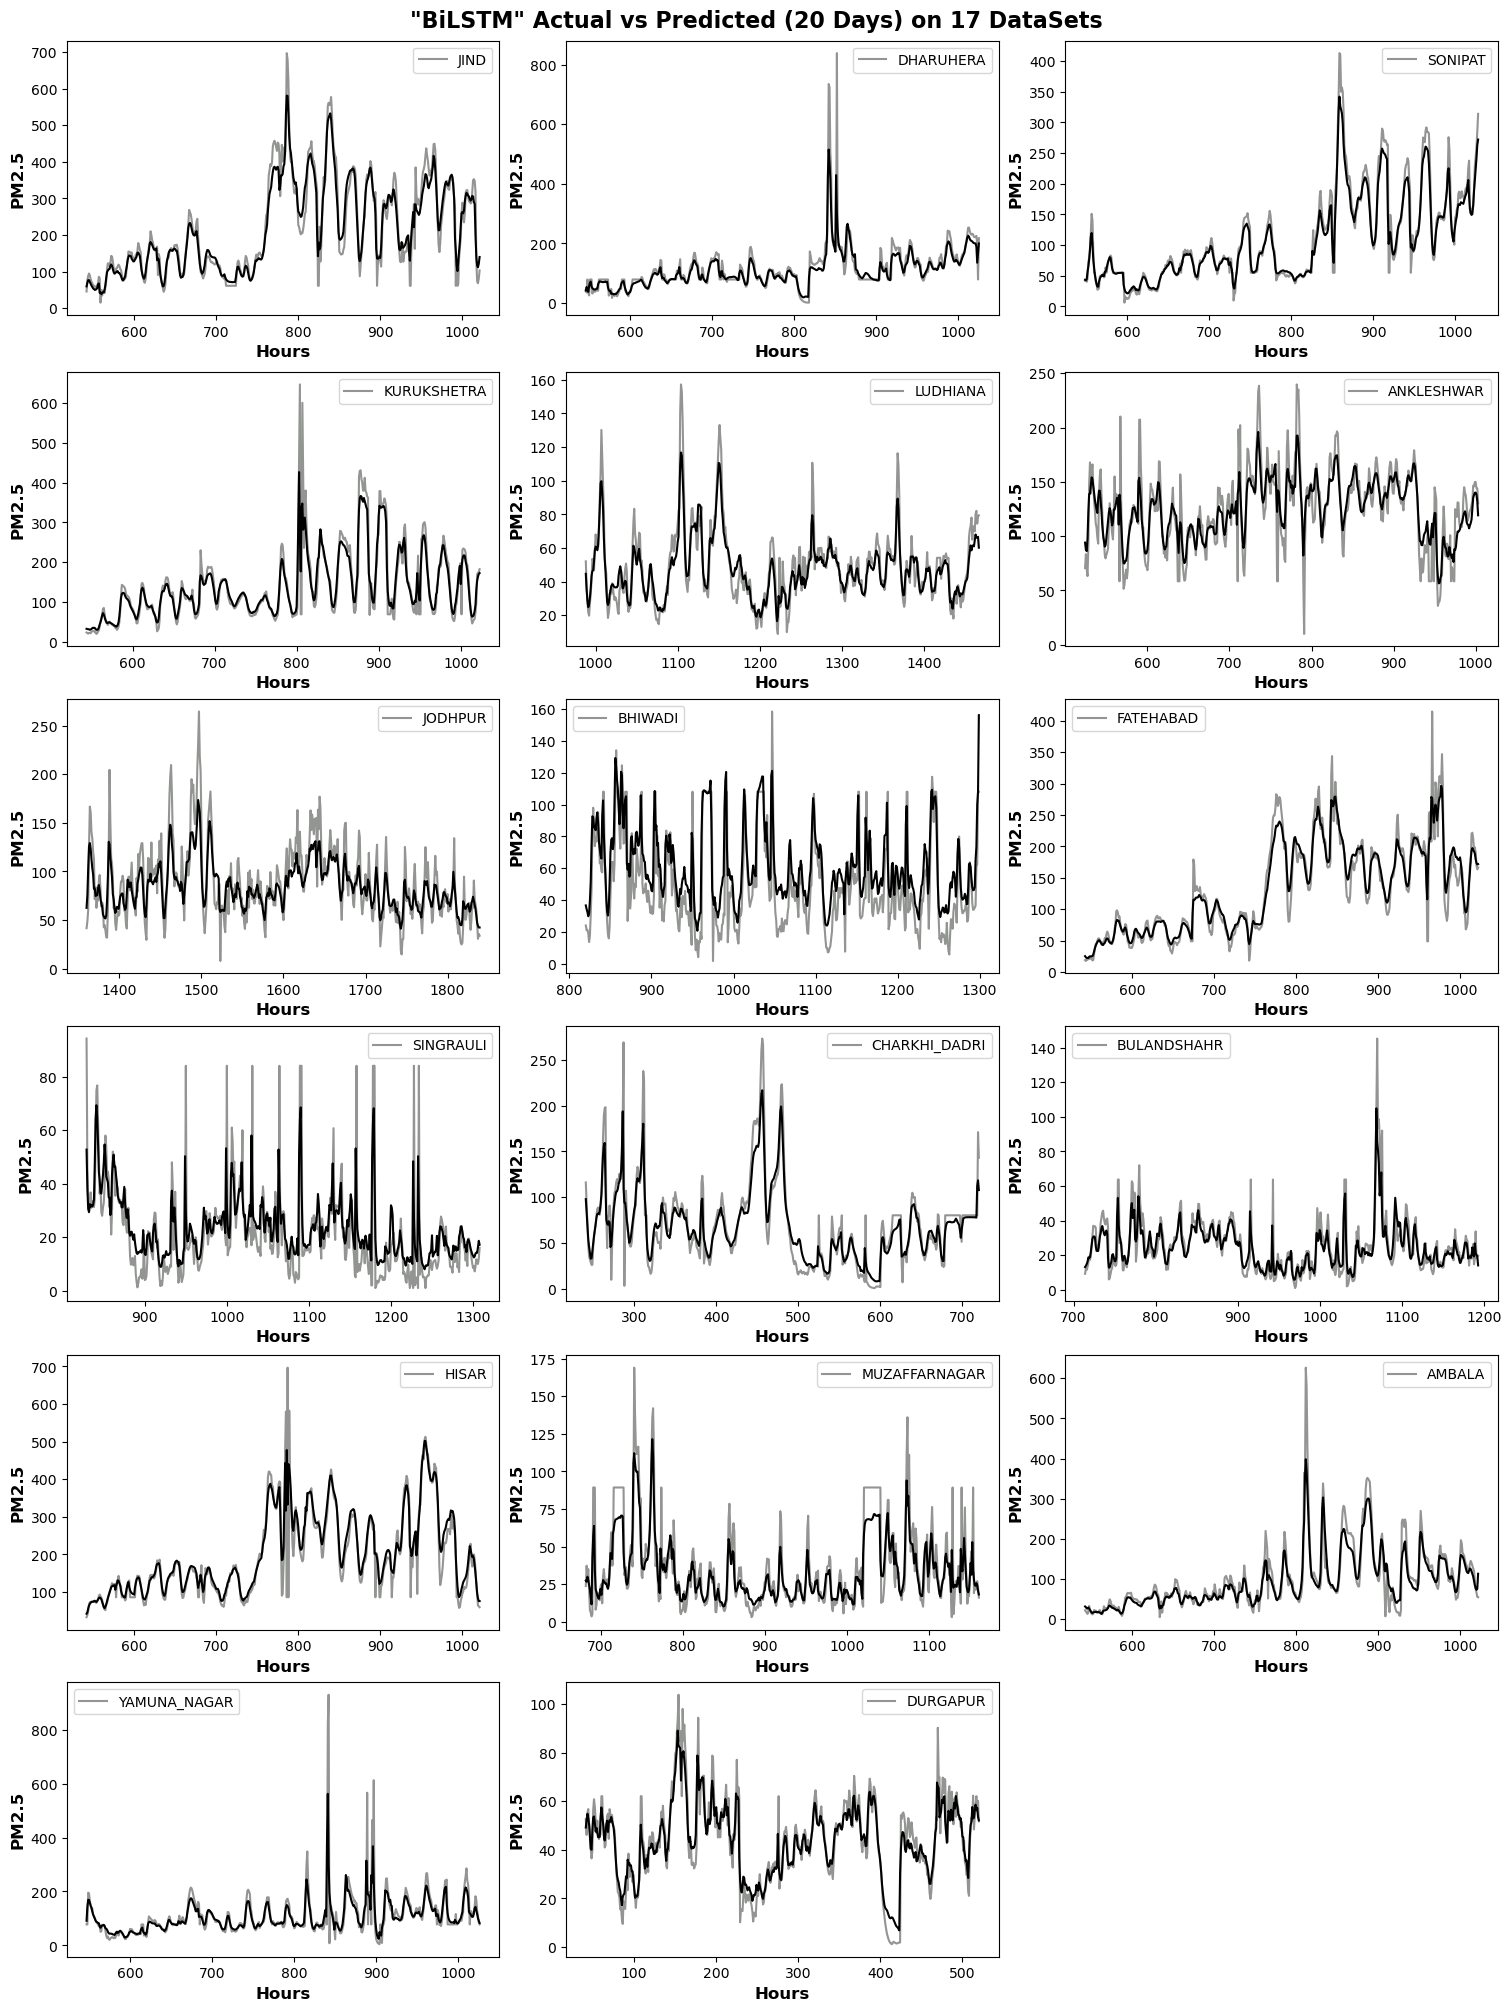
\includegraphics[width=1\textwidth]{BiLSTM(11)}
    \caption{Actual vs Predicted of BiLSTM for All Datasets}
    \label{img:bilstn_a_p}
\end{figure}

% Chapter Template

\chapter{Conclusion} % Main chapter title

\label{c6} % Change X to a consecutive number; for referencing this chapter elsewhere, use \ref{ChapterX}

\section{Conclusion}



%\include{Chapters/Chapter1}
%\include{Chapters/Chapter2} 
%\include{Chapters/Chapter3}
%\include{Chapters/Chapter4}


%-----------------------appendix---------------------
%----------------------------------------------------------------------------------------
%	THESIS CONTENT - APPENDICES
%----------------------------------------------------------------------------------------

\appendix % Cue to tell LaTeX that the following "chapters" are Appendices

% Include the appendices of the thesis as separate files from the Appendices folder
% Uncomment the lines as you write the Appendices

%% Appendix A

\chapter{Frequently Asked Questions} % Main appendix title

\label{AppendixA} % For referencing this appendix elsewhere, use \ref{AppendixA}

\section{How do I change the colors of links?}

The color of links can be changed to your liking using:

{\small\verb!\hypersetup{urlcolor=red}!}, or

{\small\verb!\hypersetup{citecolor=green}!}, or

{\small\verb!\hypersetup{allcolor=blue}!}.

\noindent If you want to completely hide the links, you can use:

{\small\verb!\hypersetup{allcolors=.}!}, or even better: 

{\small\verb!\hypersetup{hidelinks}!}.

\noindent If you want to have obvious links in the PDF but not the printed text, use:

{\small\verb!\hypersetup{colorlinks=false}!}.

%\include{Appendices/AppendixB}
%\include{Appendices/AppendixC}

%-----------------------appendix---------------------

%----------------------------------------------------------------------------------------
%	BIBLIOGRAPHY
%----------------------------------------------------------------------------------------
%\documentclass{article}
\printbibliography[heading=bibintoc]
%\bibliographystyle{IEEEtran}
%\bibliography{Bibliography.bib}
%\end{document}
%----------------------------------------------------------------------------------------

%----------------------------------------------------------------------------------------
\end{document}
